%-------------------------------LATEX SYNTAX----------------------------------
%
%   enter:              \\, \linebreak, \newline
%   new page:           \newpage
%   tab:                \tab
%   new section:        \section{name} text
%   new paragraph       \subsection{name} text  (subsub...section{name} for more layers)
%   refer:              \nameref{label name}    (place "\label{name}" at the position you want to refer to)
%   %, &, $, etc:       \%, \&, \$, etc     (these are latex operators, add a "\" to type it as text)
%   add comment:        \commred{text}, \commblue{text}, \commpurp{text}, \commgreen{text}
%   bullet points:      \begin{itemize} \item{text} ... \item{text} \end{itemize}
%   clean code:         \cleancode{text}
%   idem without indent:\cleanstyle{text}
%   bold, italic, under:\textbf{text}, textit{text}, \underline{text}
%   table:              \begin{tabular}{c c c} text \end{tabular}   ('&' for tab, '\\' for new line)
%   
%   use Google for the rest
%   
%------------------------------------------------------------------------------

\documentclass[a4paper]{article}
\usepackage[letterpaper, margin=1in]{geometry}
\usepackage{amsmath}
\usepackage{graphicx}
\usepackage{hyperref}
\usepackage{titling}
\usepackage{float}
\usepackage[utf8]{inputenc}
\usepackage{xcolor}
\usepackage{listings}
\usepackage{easylist}
\usepackage{minted}
\usepackage{tabularx}

\definecolor{lightgray}{gray}{0.9}
\pretitle{%
  \begin{center}
  \LARGE
  
\includegraphics[width=6cm,height=6cm]{images/logo}\\[\bigskipamount]
}
\posttitle{\end{center}}
\setlength{\parindent}{0cm}

\begin{document}

\title{\Huge User Manual\\Version 2.00}
\author{\\\\\\\\\\\\\\\\\\\\\\\\\\\\\\Distributed by the Potoff and Schwiebert Groups\\\textcopyright Wayne State University}

\maketitle
\thispagestyle{empty}
\newpage

\tableofcontents
\newpage

\section{Tutorial Overview}
This document will instruct a new user how to download, compile, and run the GOMC molecular simulation code.  A basic understanding of statistical physics is recommended to complete this tutorial.\\\\
To demonstrate the capabilities of the code, the user is guided through the process of downloading and compiling a GOMC executable.  That executable is then used to perform saturated vapor and liquid equilibria (VLE) studies on systems of pure isobutane (R600a), a branched alkane that whose application as a refrigerant/propellant is increasing.\\\\
\url{http://en.wikipedia.org/wiki/Isobutane}\\\\
The Transferable Potentials for Phase Equilibria (TraPPE) united atom (UA) force field is used to describe the molecular geometry constraints and the intermolecular interactions.

\section{Introduction}
Monte Carlo (MC) simulation is a type of simulation driven by stochastic processes.  "GO" stands for GPU-Optimized; this code was intended to run optimally on modern graphics process hardware.\\\\
More specifically, this engine includes serial and GPU-Optimized (multi-threaded) codes designed to run Markov chain Boltzmann sampling of chemical systems -- effectively sets of points defined by topological maps and interaction algorithms in a simulation box.  From statistical mechanics, we know this is one way to sample phase space and model chemical systems.\\\\
GOMC currently supports canonical, isobaric-isothermal, Grand canonical, constant volume Gibbs ensemble, and constant pressure Gibbs ensemble simulations.  GOMC employs widely-used simulation file types (PDB, CHARMM-style parameter file, PSF).  GOMC includes configurational bias algorithms for both linear and branched charged, and none charged systems. 

\section{How to get the software}
The latest public code builds, project logo, manual, and other resources can be obtained via the following website:\\\\
\url{http://gomc.eng.wayne.edu/}

\begin{figure}[H]
\centering
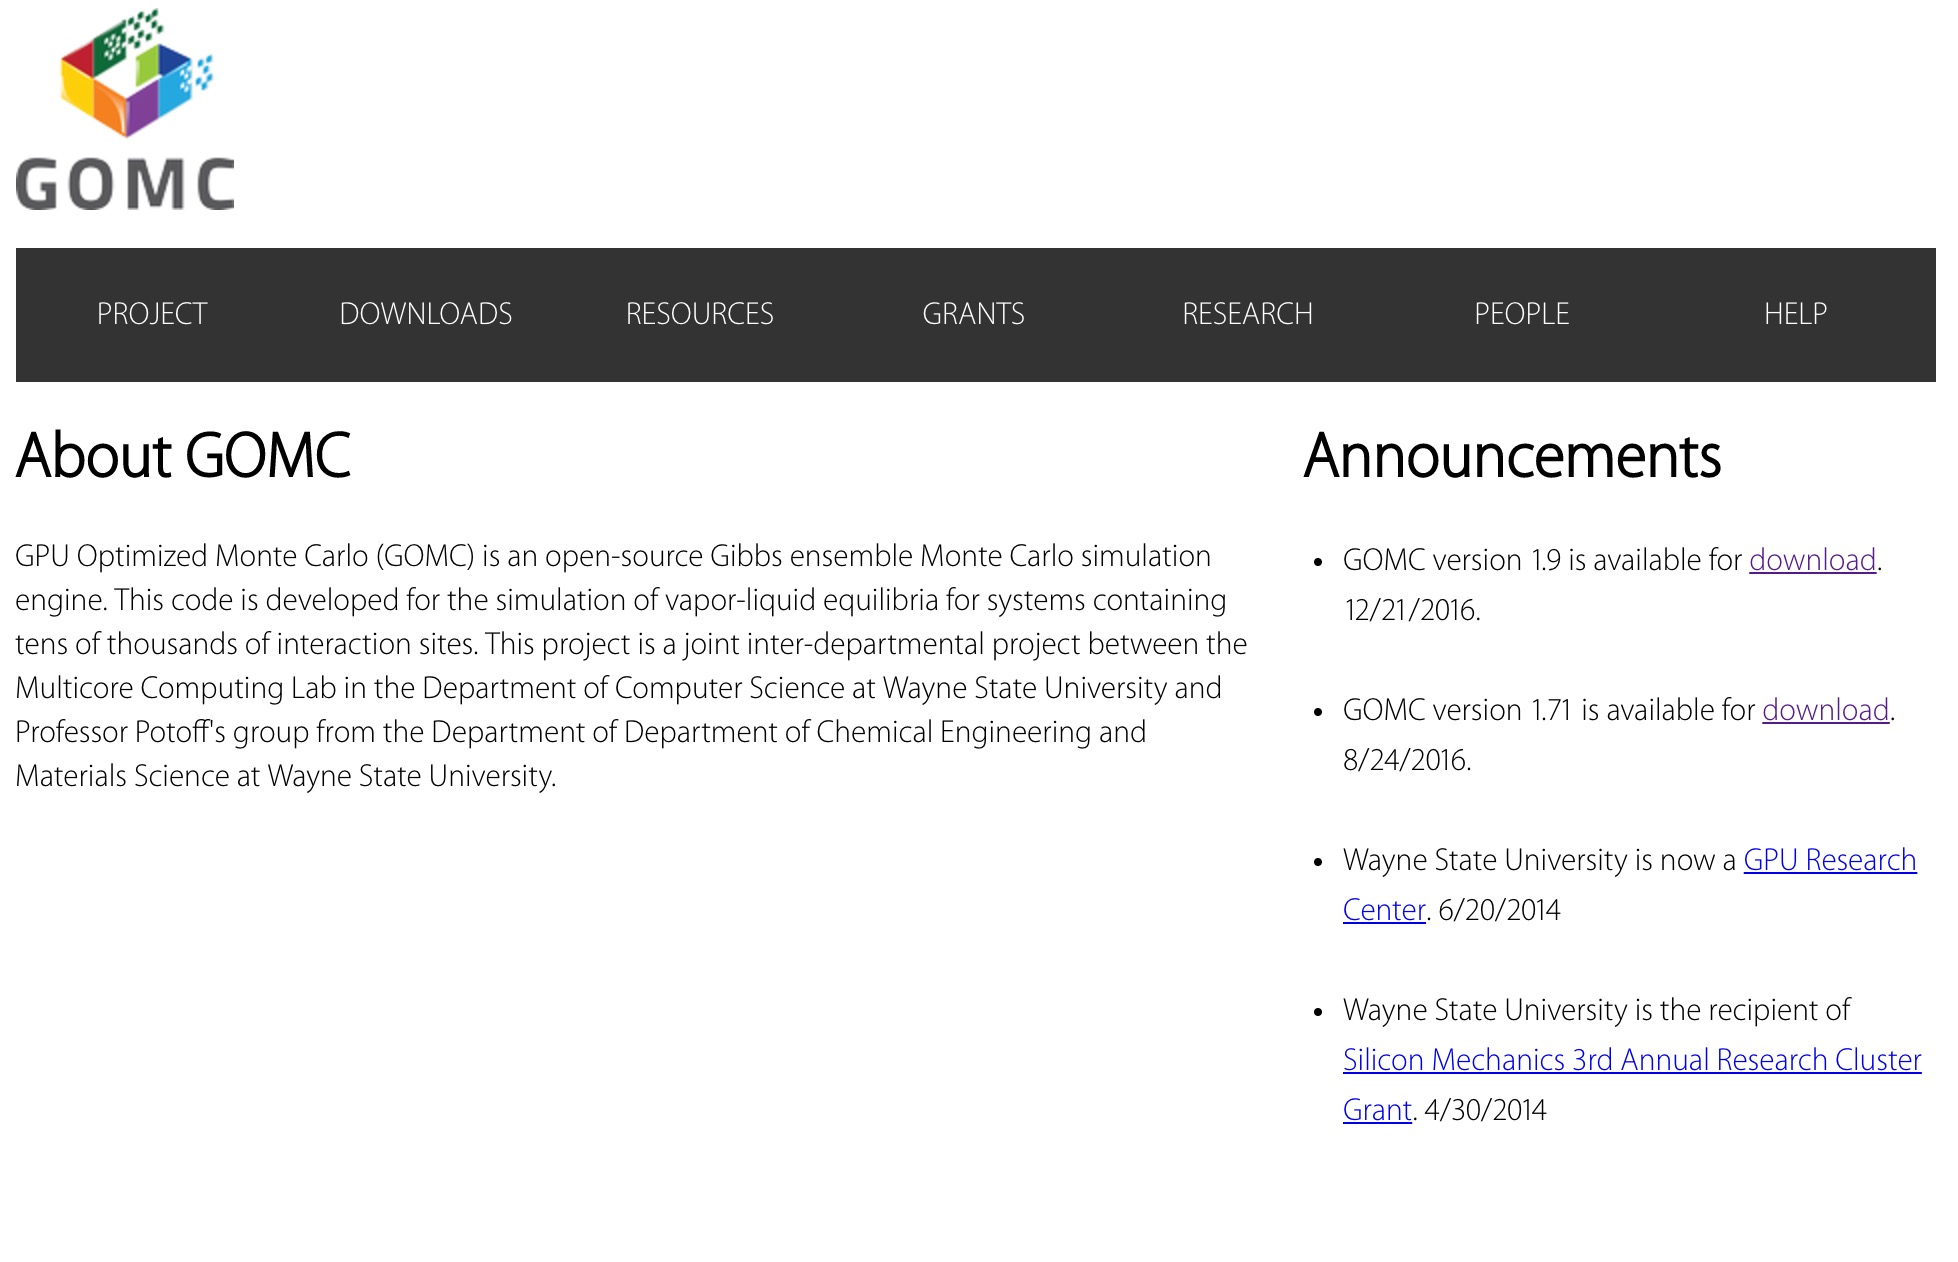
\includegraphics[scale=0.15]{images/website}
\end{figure}

The code can be found under the download tab, below and to the right of the logo.  When new betas (or release builds) are announced, they will replace the prior code under the downloads tab.  An announcement will be posted on the front page to notify users. \\\\
Currently, version control is handled through the GitHub repository.  The posted builds in Master branch are ``frozen" versions of the code that have been validated for a number of systems and ensembles. Other branches are created as a means of implementing new features. The latest updated code builds, project logo, manual, example files, and other resources can be obtained via the following GitHub repository:\\\\
\url{https://github.com/GOMC-WSU}

\begin{figure}[H]
\centering
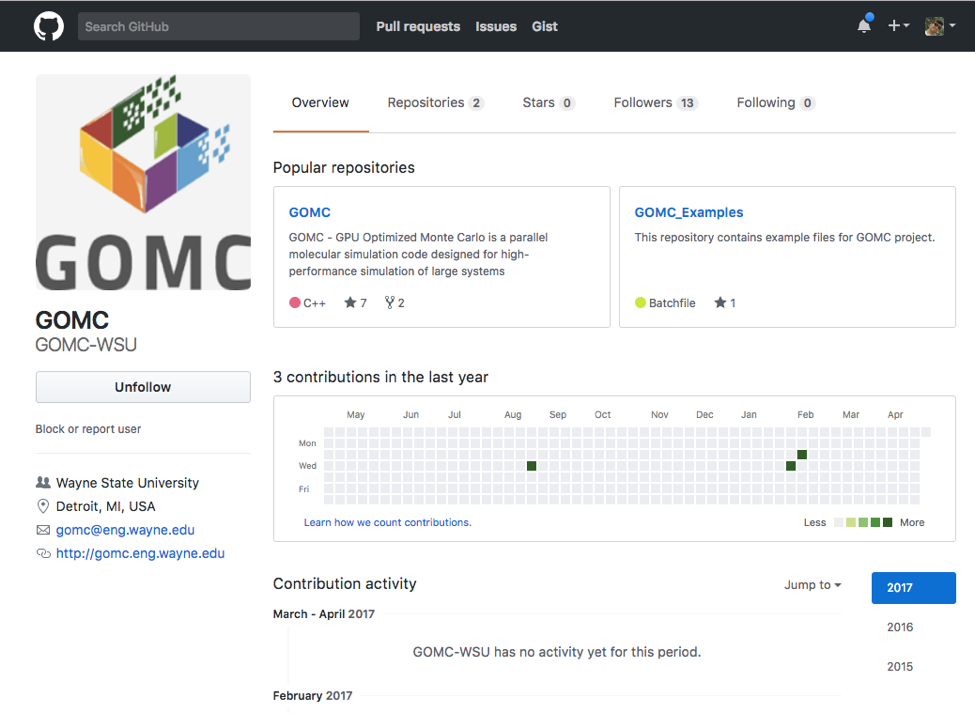
\includegraphics[scale=0.6]{images/github}
\end{figure}

The CPU and GPU code are merged together under GOMC repository and can be found under the main page. In addition, Examples repository can be found under the main page. Under each repository, the code and manual can be downloaded by clicking on the Clone or download tab. For more information regarding GitHub, visit the following link:\\\\
\url{https://guides.github.com/activities/hello-world/}

\begin{figure}[H]
\centering
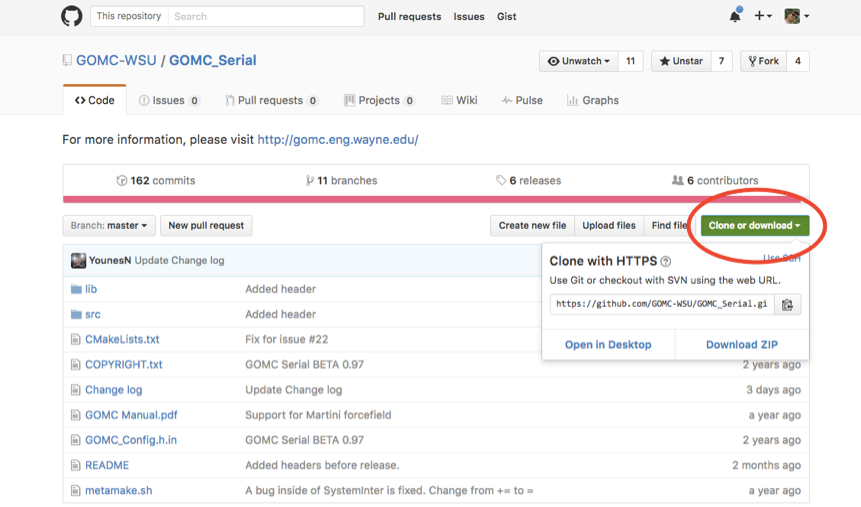
\includegraphics[scale=0.8]{images/clone}
\end{figure}

\section{Platform and Software Requirements}

\subsection{Supported Operating Systems}

GOMC officially supports Windows 7, 8, and most modern distributions of Linux (see the next section).  This software has the ability to compile on recent versions of OS X; however, such a platform is not officially supported. 

\subsection{Required Software Prequisites}

GOMC has some mild software requirements, which are widely available for Linux operating systems.  Required software requirements are:\\\\
\begin{easylist}[articletoc]
� C++03 Compliant Compiler
�� Linux/OS X
��� icc (Intel C++ Compiler)\\
Type the following command in a terminal: \\\\
\texttt{\$ icc --version} \\\\
If gives a version number 4.4 or later, you're all set.  If it's older than 4.4 (released in 2009), we recommend upgrading. \\
In Linux, the Intel compiler will generally produce the fastest serial executables (when running on Intel Core processors). \\\\
��� g++ (GNU GCC) \\
Type the following command in a terminal.\\\\
\texttt{\$ g++ --version}\\\\
If gives a version number 4.4 or later, you're all set. If it's older than 4.4 (released in 2009), we recommend upgrading.

�� Windows
��� Visual Studio\\
Microsoft's Visual Studio 2010 or later is recommended.\\
To check the version:\\
\textit{Help} (top tab) $\to$ \textit{About Microsoft Visual Studio}
\begin{figure}[H]
\centering
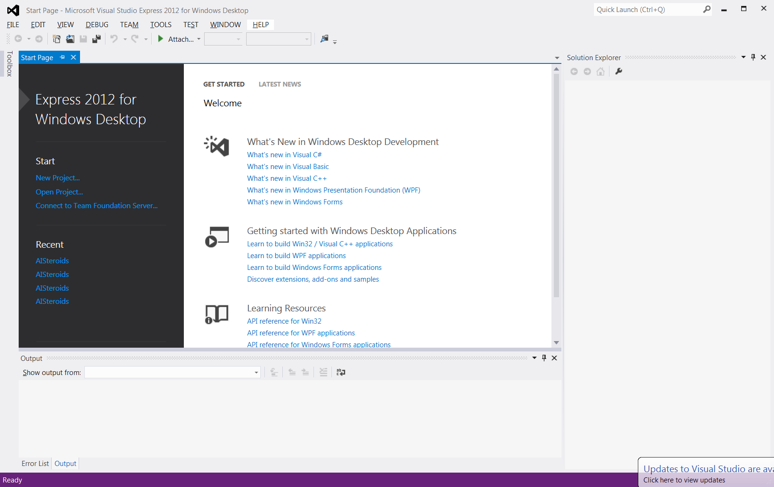
\includegraphics[scale=0.6]{images/vshelp}
\end{figure}
\begin{figure}[H]
\centering
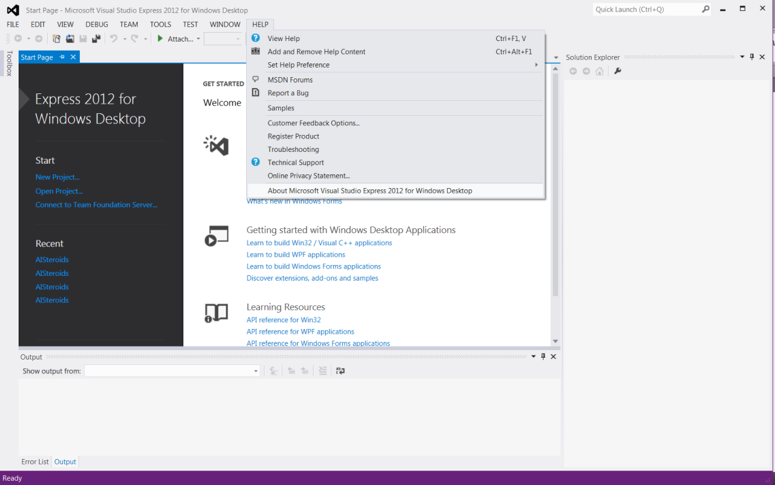
\includegraphics[scale=0.6]{images/vsabout}
\end{figure}

��� cmake (if compiling on Linux)\\
To check if cmake is installed:\\\\
\texttt{\$ which cmake}\\\\
To check the version number:\\\\
\texttt{\$ cmake --version}\\

��� nvcc/CUDA libs\\
The GPU builds of the code requires NVIDIA's CUDA 6.0 or newer:\\
To check if nvcc is installed:\\\\
\texttt{\$ which nvcc}\\\\
To check the version number:\\\\
\texttt{\$ nvcc --version}\\\\
CUDA is viewed as an essential requirement, but is not used to compile the serial code, which can be compiled on systems without CUDA.\\
To download CUDA visit NVIDIA's webpage:\\\\
\url{https://developer.nvidia.com/cuda-downloads}
\begin{figure}[H]
\centering
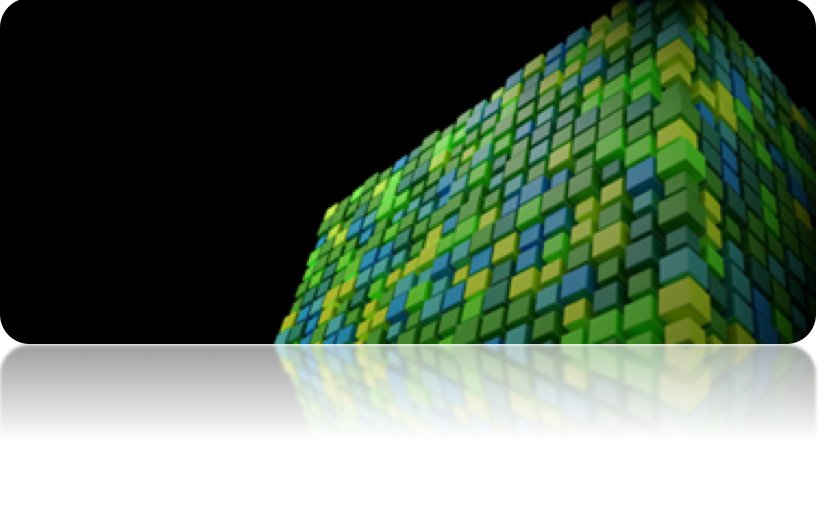
\includegraphics[scale=0.6]{images/cuda}
\end{figure}
CUDA is required to compile the GPU executable in both Windows and Linux.  Please refer to CUDA Developer webpages to select an appropriate version for the desired platform.\\
To install CUDA in Linux root/sudo, privileges are generally required.  In Windows, administrative access is required.
\end{easylist}

\section{Highly Recommended Software Tools}
\textit{\colorbox{yellow}{NOTE}: The listed programs are used in this manual and are generally considered necessary.}
\subsection{VMD}
VMD (Visual Molecular Dynamics) is a 3-D visualization and manipulation engine for molecular systems written in C-language. VMD is distributed and maintained by the University of Illinois at Urbana-Champaign.  Its sources and binaries are free to download. It comes with a robust scripting engine, which is capable of running python and tcl scripts.
More info can be found here:\\\\
\url{http://www.ks.uiuc.edu/Research/vmd/}\\\\
Although GOMC uses the same fundamental file types ? PDB (coordinates) and PSF (topology) as VMD, it uses some special tricks to obey certain rules of those file formats.\\
One useful purpose of VMD is visualization of your systems.
\begin{figure}[H]
\centering
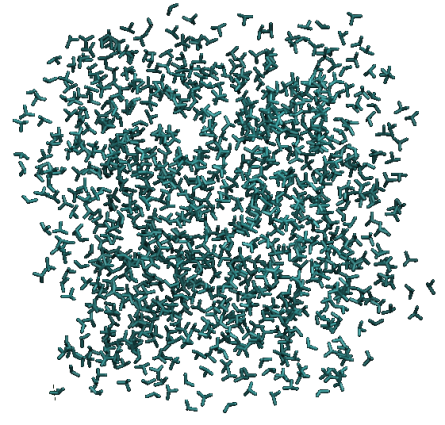
\includegraphics[scale=0.6]{images/vmd}
\caption{A system of united atom isobutane molecules}
\end{figure}
Nonetheless, the most critical part of VMD is a tool called PSFGen.  PSFGen uses a tcl or python script to generate a PDB and PSF file for a system of one or more molecules.  It is, perhaps, the most convenient way to generate a compliant PSF file.
\begin{figure}[H]
\centering
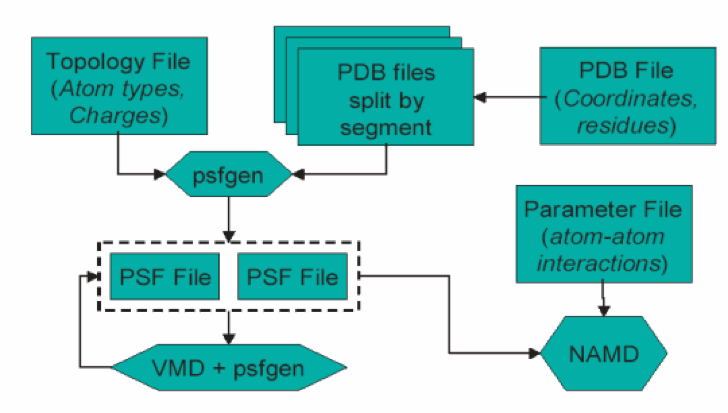
\includegraphics[scale=0.6]{images/psfgen}
\caption{An overview of the PSFGen file generation process and its relationship to VMD/NAMD}
\end{figure}
To read more about PSFGen, reference:\\\\
Plugin homepage @ UIUC\\
\url{http://www.ks.uiuc.edu/Research/vmd/plugins/psfgen}\\\\
``Generating a Protein Structure File (PSF)", part of the NAMD Tutorial from UIUC\\
\url{http://www.ks.uiuc.edu/Training/Tutorials/namd/namd-tutorial-html/node6.html}\\\\
In-Depth Overview [PDF]\\
\url{http://www.ks.uiuc.edu/Research/vmd/plugins/psfgen/ug.pdf}\\\\

\subsection{Packmol}
Packmol is a molecule packing tool created by Jos\'e Mario Mart\'inez, a professor of mathematics at the State University of Campinas, Brazil.  It is written in Fortran and is free to download.  More information is available on their homepage:\\\\
\url{http://www.ime.unicamp.br/~martinez/packmol}\\\\
To compile it, a Fortran language compiler is needed, such as gfortran.  Many Linux distributions no longer come with Fortran compilers automatically, so this may need to be installed additionally.\\
Packmol allows a specified number of molecules to be packed at defined separating distances within a certain region of space.  One of Packmol?s limitations is that it is unaware of topology; it treats each molecule or group of molecules as a rigid set of points.\\\\
\textit{\colorbox{red}{WARNING}: Another more serious limitation is that it is not aware of periodic boundary conditions (PBC).  As a result, when using Packmol to pack PDBs for GOMC, it is recommended to pack to a box 1 Angstroms smaller than the simulation box size.  This prevents hard overlaps over the periodic boundary.}

\section{Other Useful Software Tools}
\subsection{Grace}
Grace is a piece of graphing software written and maintained by the Weizmann Institute of Science's Plasma Laboratory (Rehovot, Israel). Mostly used in Linux, it can also be compiled in Windows.  The developers warn it may be missing some functionality.\\
\begin{figure}[H]
\centering

\includegraphics[scale=0.6]{images/grace}
\end{figure}
In-depth information and the source can be found on the project page, here:\\\\
\url{http://plasma-gate.weizmann.ac.il/Grace}\\\\
When compiled, Grace's executable in Linux is typically named ``xmgrace".  This tool allows the production of high quality, precise line and dot graphs, ideal for visualizing much of the thermodynamic data from the GOMC engine.  Below is an example of the results of simulations of saturated VLE densities of linear alkanes produced with Grace.
\begin{figure}[H]
\centering
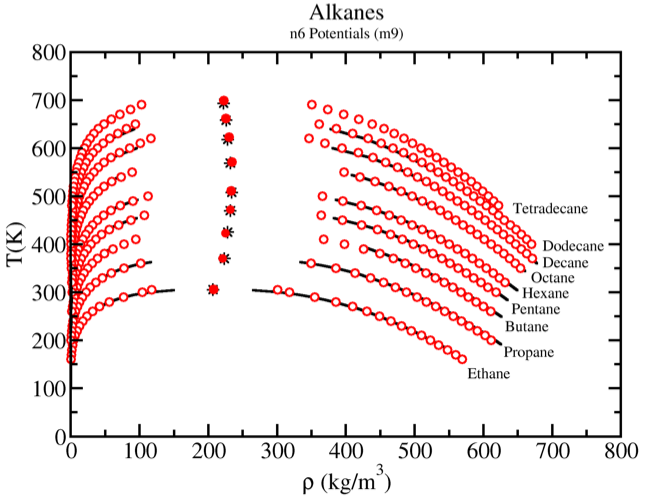
\includegraphics[scale=0.6]{images/alkanes}
\end{figure}

\subsection{Cygwin}
Cygwin is one option to assist in building and visualizing systems in Windows. It provides Microsoft Windows users with a Unix-like environment and command-line interface, and offers Windows-compatible ports of common Linux applications.\\\\
\url{https://cygwin.com}
\begin{figure}[H]
\centering
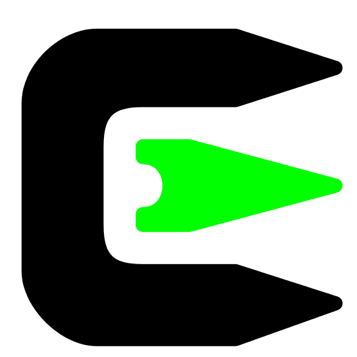
\includegraphics[scale=0.6]{images/cygwin}
\end{figure}
The software is a free and open source, licensed under the GNU General Public License version 3. Its primary maintainers are Red Hat Inc. and NetApp. One of the most impressive abilities of Cygwin is its ability to launch a full Windows-compatible X-server Window, which allows convenient visualization of Linux app GUIs. It is compatible with the Grace graphing software. In practice, this package behaves most analogously to a Linux virtual machine in Windows.

\section{Compiling GOMC}
\subsection{Extracting the code}
GOMC is distributed as a compressed folder, containing the source and build system. To compile the code after downloading it, the first step is to extract the compressed build folder.\\
In Windows, the folder for the GPU code is compressed using a standard *.zip file format. To unzip simply use a utility like Peazip: \\\\
\url{http://peazip.sourceforge.net/}\\\\
Below is an example of what the downloaded code looks like when unzipping in Peazip.
\begin{figure}[H]
\centering
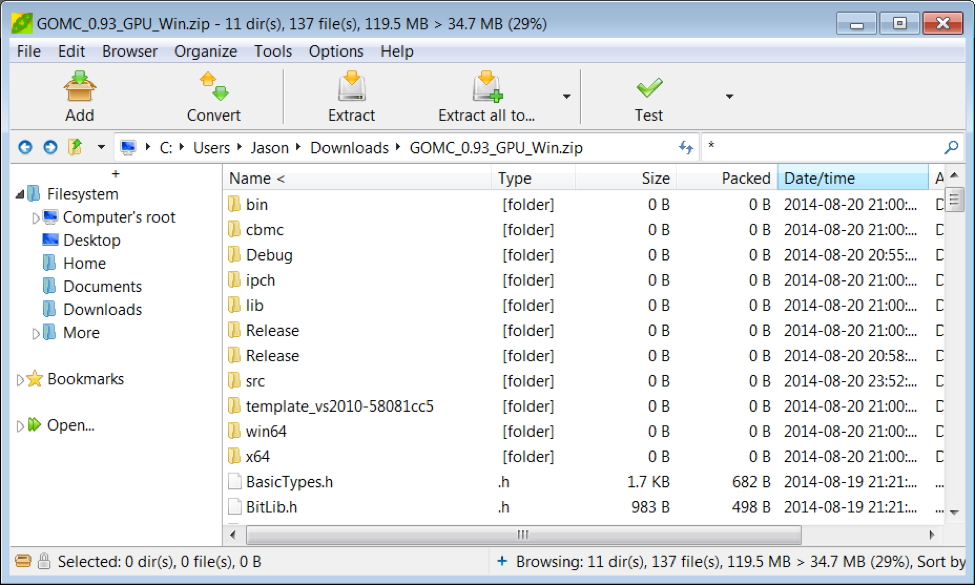
\includegraphics[scale=0.6]{images/peazip}
\end{figure}
In Linux, the GPU and Serial codes are compressed using gzip and tar (*.tar.gz).  To extract, simply move to the desire folder and type in the command line:\\\\
\texttt{\$ tar -xzvf <file name>.tar.gz}
\subsection{Compiling the code}
\subsubsection{GPU code}
\underline{Compilation on Windows}\\
Once the code is extracted, to compile it on Windows, you need to load the project into Visual Studio by opening the extracted folder and double clicking on the solution file of the desired Visual Studio version.  After the solution is opened in Visual Studio, go to the ``Build" menu and select ``Build solution" to compile the code. You can compile either with release mode or with debug mode by selecting the desired mode from the ``Solution Configuration" drop box. 
To run the project, simply click the run button or hit F5 on the keyboard.\\\\
\underline{Compilation on Linux}\\
To compile the GPU code on Linux, go to the directory of the project, and type in the command line:\\\\
\texttt{\$ make}\\\\
You can configure the ``makefile" file to choose different C compilers, to select the desired compute capability, and to configure many more compilation flags.\\
The default compute capability is 3.0. To change the compute capability, go to the \texttt{GENCODE\_FLAGS} option, and set it to one of the compute capability flags that are defined in the file.
\begin{minted}[frame=single,framesep=10pt]{make}
# CUDA code generation flags
GENCODE_SM10    := -gencode arch=compute_10,code=sm_10
GENCODE_SM10    := -gencode arch=compute_20,code=sm_20
GENCODE_SM10    := -gencode arch=compute_30,code=sm_30
GENCODE_SM10    := -gencode arch=compute_35,code=sm_35
GENCODE_FLAGS   := $(GENCODE_SM30)
\end{minted}
To run the program, run the executable ``GOMC.out".  The system's \texttt{LD\_LIBRARY\_PATH} will need to be configured to support CUDA (more on this later).
\subsubsection{Serial Code}
\underline{Compilation on Windows}\\
See GPU ``Compilation on Windows" section and follow an identical procedure for the released serial code. See \texttt{README} for instructions on how to use the CMake-GUI to build the configuration and solution files necessary for the Windows build.\\\\
\underline{Compilation on Linux}\\
In Linux, the CPU code uses a simple makefile. Enter the directory and type in the command line:\\\\
\texttt{\$ make all}\\\\
This will use the Makefile to compile a GPU-compatible executable called ``GOMC.out".  To run, the system?s \texttt{LD\_LIBRARY\_PATH} will need to be configured to support CUDA (more on this later).
For the serial code, which uses cmake for compilation, go to the base directory and type in the command line:\\\\
\texttt{\$ ./metamake.sh}\\\\
This cmake script will create a directory named ``bin".  Enter this directory:\\\\
\texttt{\$ cd bin}\\\\
and type:\\\\
\texttt{\$ make}\\\\
Four executables - \texttt{GOMC\_Serial\_GEMC} (Gibbs ensemble), \texttt{GOMC\_Serial\_NVT} (NVT ensemble), \texttt{GOMC\_Serial\_NPT} (isobaric-isothermal ensemble), and \texttt{GOMC\_Serial\_GCMC} (Grand canonical ensemble) - will be produced. By default, the distribution compiles in release mode.  To compile in debug mode (if you're using the code as a developer), open the file ``\texttt{CMakeCache.txt}" while still in the ``bin" folder.  This file contains information used by cmake to build the executables.  To compile in debug mode, change the value after ``\texttt{CMAKE\_BUILD\_TYPE:STRING=}" from ``Release" to ``Debug", and retype the command:\\\\ \texttt{\$ make}\\\\
The output executables should now be compiled with debugger symbols.
You can also swap the compiler by modifying the ``\texttt{CMAKE\_CXX\_COMPILER}" variable. For more information, refer to the CMake documentation.\\
Running GOMC in parallel using OpenMP:\\
To run the parallel version of CPU code, it needs to be compiled with openmp library. Open the file ``\texttt{CMakeCache.txt}", while still in the ``bin" folder, and change the value after ``\texttt{CMAKE\_CXX\_FLAGS\_RELEASE:STRING=}" from ``-O3 -DNDEBUG" to ``-O3 -qopenmp -DNDEBUG".\\
And retype the command:\\\\
\texttt{\$ make}\\\\
\section{Input File Formats}
In order to run simulation in GOMC, the following files need to be provided:
\begin{itemize}
\item GOMC executable
\item Input file ``NAME.conf" (proprietary control file)
\item PDB file(s)
\item PSF file(s)
\item Parameter file
\end{itemize}
\subsection{PDB File}
The PDB file stores coordinates for the simulation. The file format is widely adopted.
\begin{itemize}
\item Protein Databank (PDB) Files (plural: PDB files)
\item Open format, well-documented
\item Fixed-width format (hence white space is significant)
\item Up to 13.5m page views a month; up to 55.8m FTP requests per month
\item Used by NAMD, GROMACS, CHARMM, ACEMD, Amber
\end{itemize}
An overview of the PDB standard can be found here:\\\\
\url{http://www.wwpdb.org/docs.html}\\\\
The advantage of PDB files is their ubiquity and thorough documentation. Disadvantages include limited fixed point floating precision for coordinates, unused space, and proprietary implementations creating inconsistencies.\\
One PDB file is required per box. For NVT ensemble simulations, one file is expected; for Gibbs and grand canonical ensemble, two files are required.
GOMC recognizes the following keywords in PDB files:
\begin{itemize}
\item[$\diamondsuit$] \texttt{REMARK}
\item[$\diamondsuit$] \texttt{CRYST1}
\item[$\diamondsuit$] \texttt{ATOM}
\item[$\diamondsuit$] \texttt{END}
\end{itemize}
Currently, REMARK is ignored. Formerly, it was used to store proprietary information in frames (e.g. step number). Packmol typically leaves the following remark:\\\\
\begin{tabularx}{\textwidth}{| X | X | X | X | X | X |}
\hline
  \texttt{REMARK} & \texttt{original} & \texttt{generated} & \texttt{coordinate} & \texttt{pdb} & \texttt{file}  \\
\hline
\end{tabularx}\\\\
at the top of the file. Note that this is another example of an inconsistency with the spec. As of the PDB v3.30 specification the \texttt{REMARK} entry contains an identifying integer, which is supposed to occupy lines 8-10.\\
\begin{figure}[H]
\centering
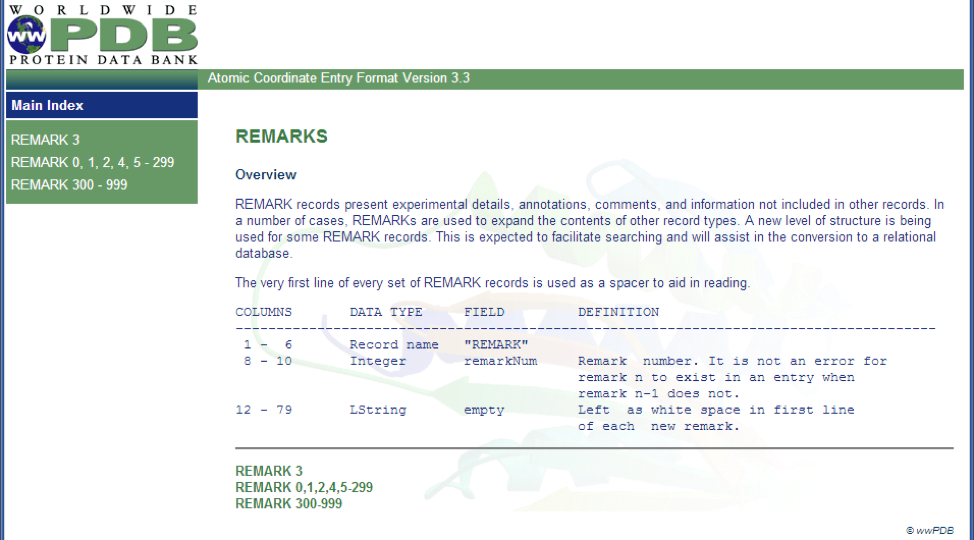
\includegraphics[scale=1.0]{images/remark}
\end{figure}
A file generated by Packmol has ``ori" in this position. Hence you may see future codes that are incompatible with this legacy kind of remarks.\\
Note also that the spaces 7 and 11 are not reserved; hence, they may be used in proprietary specifications.\\
\texttt{CRYST1} can be used to store the cell dimensions, which can also be put as a tag in the proprietary control file.\\
\url{http://www.wwpdb.org/documentation/format33/sect8.html#CRYST1}\\
\begin{figure}[H]
\centering
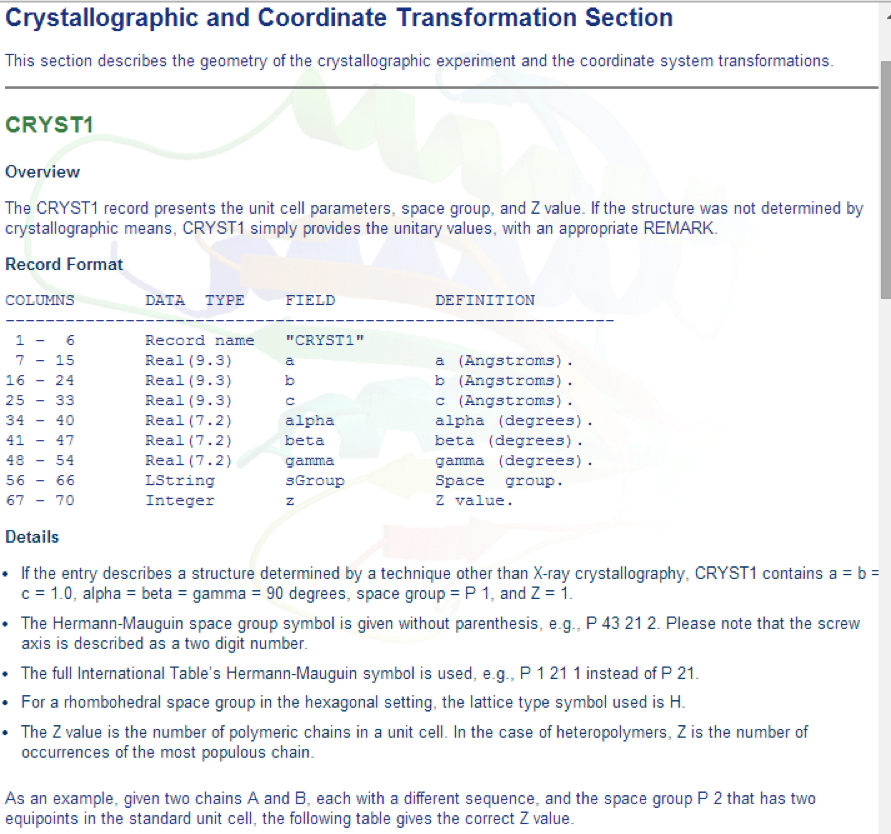
\includegraphics[scale=1.0]{images/pdb}
\end{figure}

%%%%% TODOOOOOOO 

\textit{\colorbox{yellow}{NOTE}: Only cubic and orthogonal cells are supported in this code.}
The main entry in the PDB file are \texttt{ATOM|} entries.  The keyword ``\texttt{ATOM}" is always followed by two spaces. An entry has a number of fields.
\begin{figure}[H]
\centering
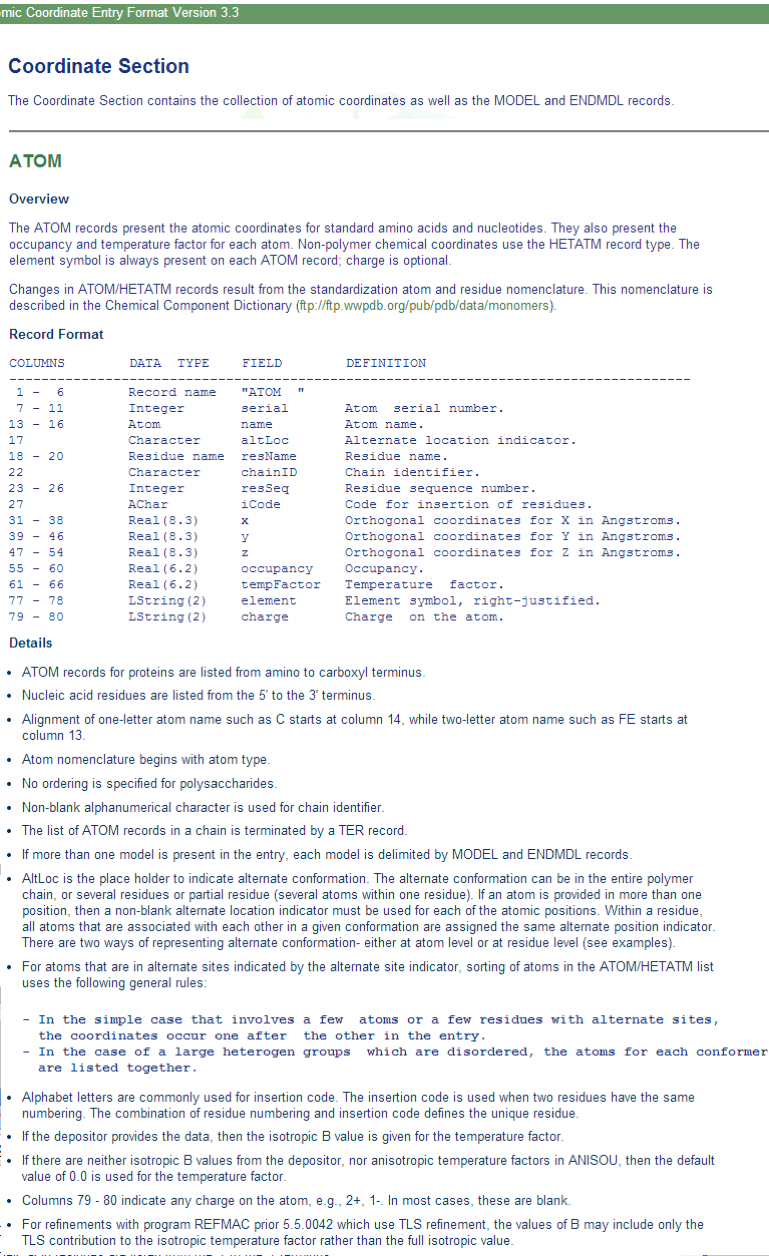
\includegraphics[scale=1.0]{images/atom}
\end{figure}
The key parameters are the coordinates x, y, and z. The precision is limited to eight whole decimal digits and three fractional decimal digits.\\
Other important entries are the residue name, atom name, and chain ID. Numbering is important primarily because it represents an inconvenience in packing/loading large systems. Revisiting the previous example,\\\\

%%%%% TODOOOOOOO

the atom name is ``C1" and residue name is ``ISB". The PSF file (next section) contains a lookup table of atoms. These contain the atom name from the PDB and the name of the atom kind in the parameter file it corresponds to. As multiple different atom names will all correspond to the same parameter, these can be viewed ``atom aliases" of sorts.  The chain letter (in this case `A') is sometimes used when packing a number of PDBs into a single PDB file.\\

A few important \colorbox{yellow}{Notes}/\colorbox{red}{Warnings} on Undocumented PDB Format Conventions:
\begin{itemize}
\item While it is explicitly stated in some other sections of the PDB file, the general convention observed by most codes is to right align when padding with white space.
\item Some codes (including PSFGen/VMD) use the 21st unused character to add a fourth letter to the residue (molecule name). This extension is currently supported, but is unofficial and, hence, may change in the future.
\item VMD requires a constant number of ATOMs in a multi-frame PDB (multiple records terminated by ``END" in a single file). To compensate for this, all atoms from all boxes in the system are written to the output PDBs of this code.
\item For atoms not currently in a box, the coordinates are set to $<0.00, 0.00, 0.00>$
\item The occupancy is commonly just set to ``1.00" and is left unused by many codes. We recycle this legacy parameter by using it to denote, in our output PDBs, the box a particle is in (box 0  occupancy=0.00 ; box 1  occupancy=1.00)
\item As the x, y, and z coordinates are fixed point with only three digits of precision, the energy values you get when restarting may be mildly different, particularly for bonded interactions due to roundoff in the coordinates.  This will eventually be remedied by the implementation of a full-precision trajectory (e.g. DCD) file.
\item The ``ISB" entry in columns 73-75 is not an official part of the PDB standard.  This is a proprietary entry called ``Segname", which has been embraced by NAMD and some other codes.
\end{itemize}
A frame in the PDB file is terminated with the keyword \texttt{END}.\\
With that overview of the format in mind, the following steps describe how a PDB file is typically built.\\
\begin{enumerate}
\item A single molecule PDB is obtained. In this example, the QM software package Gaussian was used to draw the molecule, which was then edited by hand to adhere to the PDB spec properly. The end result is a PDB for a single molecule:\\\\
\colorbox{lightgray}{
\begin{tabular}{*9l }
  \texttt{REMARK} & \multicolumn{8}{l}{\texttt{1 File created by GaussView 5.0.8}}  \\
  \texttt{ATOM} & \texttt{1} & \texttt{C1} & \texttt{ISB} & \texttt{1} & \texttt{0.911} & \texttt{-0.313} & \texttt{0.000} & \texttt{C} \\
  \texttt{ATOM} & \texttt{2} & \texttt{C2} & \texttt{ISB} & \texttt{1} & \texttt{1.424} & \texttt{-1.765} & \texttt{0.000} & \texttt{C} \\
  \texttt{ATOM} & \texttt{3} & \texttt{C3} & \texttt{ISB} & \texttt{1} & \texttt{-0.629} & \texttt{-0.313} & \texttt{0.000} & \texttt{C} \\
  \texttt{ATOM} & \texttt{4} & \texttt{C4} & \texttt{ISB} & \texttt{1} & \texttt{1.424} & \texttt{0.413} & \texttt{-1.257} & \texttt{C} \\
  \multicolumn{9}{l}{\texttt{END}} \\
\end{tabular}
}
\item Next, packings are calculated to place the simulation in a region of vapor-liquid coexistence. There are a couple of ways to do this in Gibbs ensemble:
\begin{itemize}
\item Pack both boxes to a single ?middle? density, which is an average of the liquid and vapor densities.
\item Same as 1, but add a modest amount to axis of one box (e.g. 10-30 A).  This technique can be handy in the constant pressure Gibbs ensemble.
\item Pack one box to the predicted liquid density and the other to the vapor density.
\end{itemize}
\begin{figure}[H]
\centering
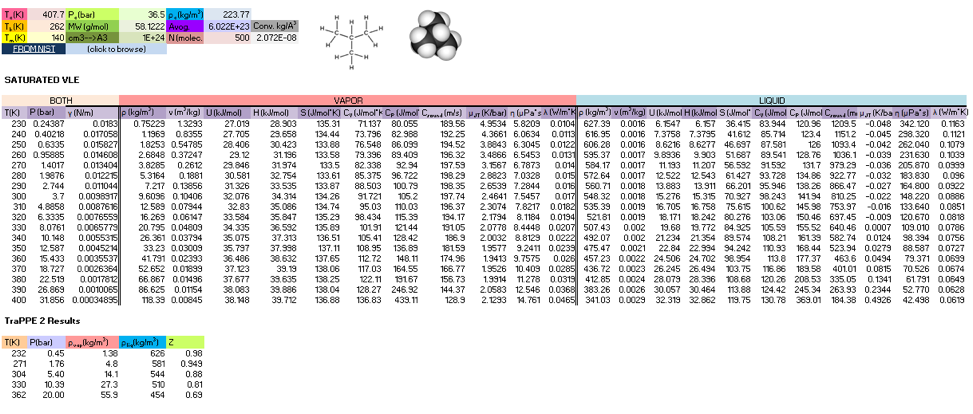
\includegraphics[scale=1.0]{images/pack2}
\end{figure}
A good reference for getting the information needed to estimate packing is the NIST Web Book database of pure compounds:\\\\
\url{http://webbook.nist.gov/chemistry/}\\\\
\item After packing is determined, a basic pack can be performed with a Packmol script.  Here is one example:\\\\
\colorbox{lightgray}{
\begin{tabular}{l}
\texttt{tolerance 3.0}\\
\texttt{filetype pdb}\\
\texttt{output STEP2\_ISB\_packed\_BOX\_0.pdb}\\\\
\texttt{structure isobutane.pdb}\\
\texttt{number 1000}\\
\texttt{inside box 0.1 0.1 0.1 70.20 70.20 70.20}\\
\texttt{end structure}
\end{tabular}
}\\\\
Packmol scripts are typically saved with the extension \texttt{*.inp}, so this might be named ``\texttt{pack\_isobutane.inp}".\\
To run the script, we type the following line into the terminal:\\\\
\texttt{\$ ./packmol < pack\_isobutane.inp}\\\\
\end{enumerate}
\subsection{PSF File}
The PSF file stores the topology, mass, charges, and atom identities of molecules in the system.
\begin{itemize}
\item Protein Structure File (PSF) 
\item Space-separated file
\item Used by NAMD, CHARMM, X-PLOR
\end{itemize}
The PSF file is not as robustly documented as the PDB format, but a basic description of it can be found here:\\\\
\url{http://www.ks.uiuc.edu/Training/Tutorials/namd/namd-tutorial-win-html/node24.html}\\\\
The PSF file is generally composed of a series of sections. A line with a numeric value is typically at the top of each section. This value lists the number of entries in that section (lines can contain multiple entries; a dihedral, for example has two quadruplet entries of atom indices per line). Note that outside the remarks and atom section, this number is typically smaller than the number of lines by a factor of 2 to 4.\\\\
PSF files always start with the string ``PSF" on their first line.\\\\
GOMC reuses PSF reading code from NAMD, hence it should have much of the same flexibility and limitations.  By section, the segments of a PSF file are:
\begin{itemize}
\item TITLE: remarks on the file
\item BONDS: the bonds (if applicable) in molecules 
\item ANGLE: the bonds (if applicable) in molecules
\item DIHEDRAL: the bonds (if applicable) in molecules
\item IMPROPER: the bonds (if applicable) in molecules
\item (other sections such as cross terms)
\end{itemize}
The code currently skips the title section and reads the bonds, angles, dihedrals and impropers.\\\\
A few important \colorbox{yellow}{Notes}/\colorbox{red}{Warnings}:
\begin{itemize}
\item The PSF file format is a highly redundant file format.  It repeats identical topology of thousands of molecules of a common kind in some cases. GOMC follows the same approach as NAMD, allowing this excess information externally and compiling it in the code.
\item Other sections (e.g. cross terms) contain unsupported or legacy parameters and are ignored.
\item Following the restrictions of VMD, the order of the PSF atoms must match the order in the PDB file.
\item Improper entries are read and stored, but are not currently used.  Support will eventually be added for this.
\end{itemize}
The PSF file is typically generated using PSFGen. It is convenient to make a script, such as the example below, to do this:\\\\
\colorbox{lightgray}{
\begin{tabular}{l}
\texttt{psfgen << ENDMOL}\\
\texttt{topology ./Top\_branched\_Alaknes.inp}\\
\texttt{segment ISB\{}\\
\texttt{    pdb ./STEP2\_ISB\_packed\_BOX\_0.pdb}\\
\texttt{    first none}\\
\texttt{    last none}\\
\texttt{\}}\\\\
\texttt{coordpdb ./STEP2\_ISB\_packed\_BOX\_0.pdb ISB}\\\\
\texttt{writepsf ./STEP3\_START\_ISB\_sys\_BOX\_0.psf}\\
\texttt{writepdb ./STEP3\_START\_ISB\_sys\_BOX\_0.pdb}\\
\end{tabular}
}\\\\
Typically, one script is run per box to generate a finalized PDB/PSF for that box. The script requires one additional file, the NAMD-style topology file. While GOMC does not directly read or interact with this file, it's typically used to generate the PSF and, hence, is considered one of the integral file types. It will be briefly discussed in the following section.\\\\

Here's a peek at how the generated PSF file looks for a packed isobutane system (abridged):\\\\
\colorbox{lightgray}{
\begin{tabular}{r l l l l l l l l}
\multicolumn{9}{l}{\texttt{PSF}}\\
\texttt{3} & \multicolumn{8}{l}{\texttt{!NTITLE}} \\
\texttt{REMARKS} & \multicolumn{8}{l}{\texttt{original generated structure x-plor psf file}}\\
\texttt{REMARKS} & \multicolumn{8}{l}{\texttt{topology ./Top\_Branched\_Alkanes.inp}}\\
\texttt{REMARKS} & \multicolumn{8}{l}{\texttt{segment ISB \{ first NONE; last NONE; auto angles dihedrals \}}}\\\\
\texttt{4000} & \multicolumn{8}{l}{\texttt{!NATOM}}\\
\texttt{1} & \texttt{ISB} & \texttt{1} & \texttt{ISB} & \texttt{C1} & \texttt{CH1} & \texttt{0.000000} & \texttt{13.0190} & \texttt{0}\\
\texttt{2} & \texttt{ISB} & \texttt{1} & \texttt{ISB} & \texttt{C2} & \texttt{CH3} & \texttt{0.000000} & \texttt{15.0350} & \texttt{0}\\
\texttt{3} & \texttt{ISB} & \texttt{1} & \texttt{ISB} & \texttt{C3} & \texttt{CH3} & \texttt{0.000000} & \texttt{15.0350} & \texttt{0}\\
\texttt{4} & \texttt{ISB} & \texttt{1} & \texttt{ISB} & \texttt{C4} & \texttt{CH3} & \texttt{0.000000} & \texttt{15.0350} & \texttt{0}\\
\texttt{5} & \texttt{ISB} & \texttt{2} & \texttt{ISB} & \texttt{C1} & \texttt{CH1} & \texttt{0.000000} & \texttt{13.0190} & \texttt{0}\\
\texttt{6} & \texttt{ISB} & \texttt{2} & \texttt{ISB} & \texttt{C2} & \texttt{CH3} & \texttt{0.000000} & \texttt{15.0350} & \texttt{0}\\
\texttt{7} & \texttt{ISB} & \texttt{2} & \texttt{ISB} & \texttt{C3} & \texttt{CH3} & \texttt{0.000000} & \texttt{15.0350} & \texttt{0}\\
\texttt{8} & \texttt{ISB} & \texttt{2} & \texttt{ISB} & \texttt{C4} & \texttt{CH3} & \texttt{0.000000} & \texttt{15.0350} & \texttt{0}\\
\multicolumn{9}{l}{\texttt{.}}\\
\multicolumn{9}{l}{\texttt{.}}\\
\multicolumn{9}{l}{\texttt{.}}\\
\texttt{3997} & \texttt{ISB} & \texttt{1000} & \texttt{ISB} & \texttt{C1} & \texttt{CH1} & \texttt{0.000000} & \texttt{13.0190} & \texttt{0}\\
\texttt{3998} & \texttt{ISB} & \texttt{1000} & \texttt{ISB} & \texttt{C2} & \texttt{CH3} & \texttt{0.000000} & \texttt{15.0350} & \texttt{0}\\
\texttt{3999} & \texttt{ISB} & \texttt{1000} & \texttt{ISB} & \texttt{C3} & \texttt{CH3} & \texttt{0.000000} & \texttt{15.0350} & \texttt{0}\\
\texttt{4000} & \texttt{ISB} & \texttt{1000} & \texttt{ISB} & \texttt{C4} & \texttt{CH3} & \texttt{0.000000} & \texttt{15.0350} & \texttt{0}\\

\end{tabular}
}\\\\


















\end{document}